\chapter{Introdução}

\section{Contexto de Pesquisa}

\section{Declaração do Problema}

\section{Objetivos de Pesquisa}


\section{Contribuições de pesquisa}


\section{Publicações}

\section{Metodologia de Pesquisa}

\begin{figure}
    \centering
    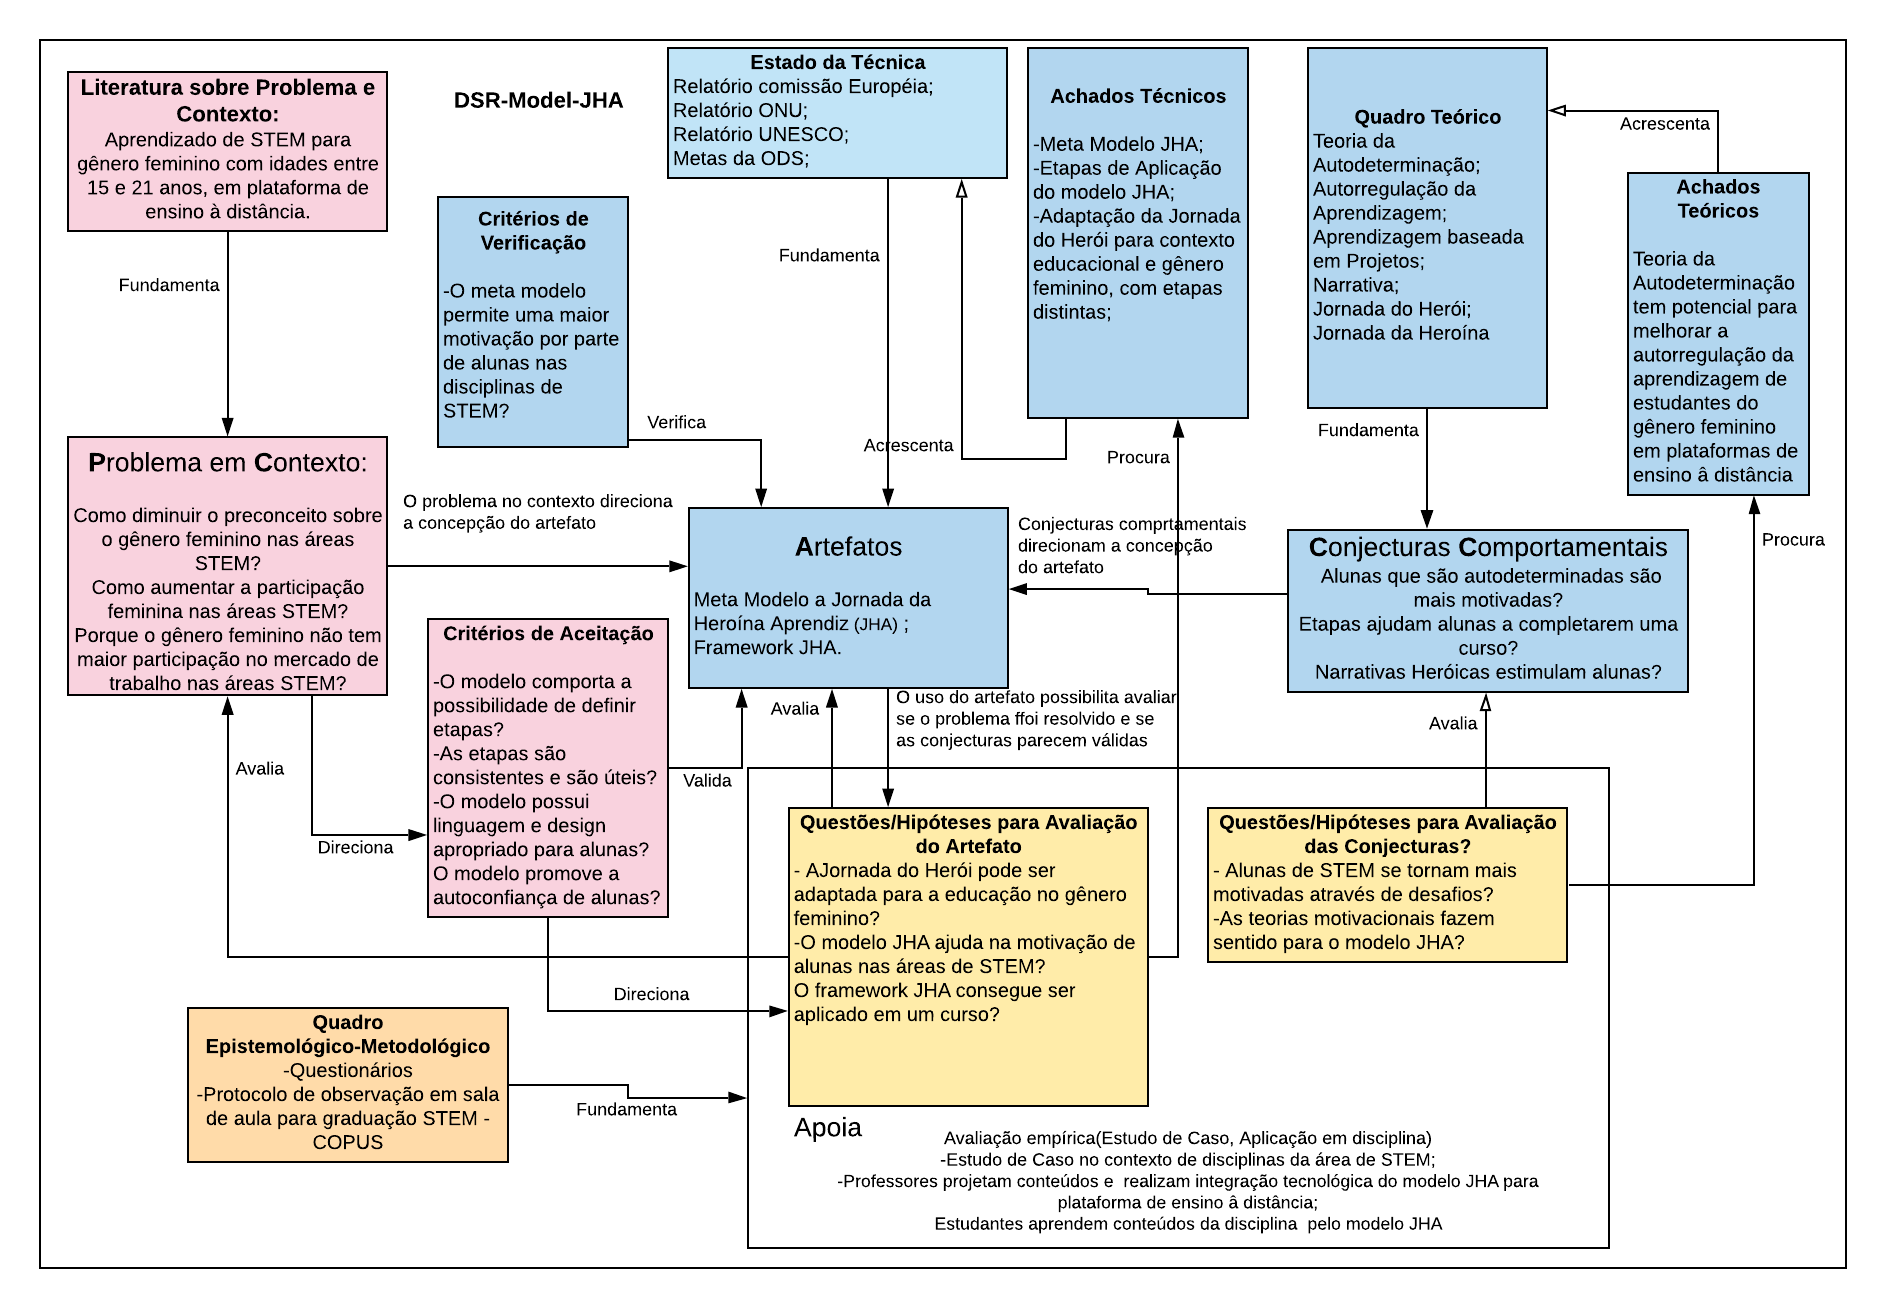
\includegraphics[width=.9\textwidth]{chaps/Images/DSRV2.png}
    \caption{Design Science Research}
    \label{fig:dsr}
\end{figure}

Uma das questões de pesquisa que importa para este estudo é: Como motivar estudantes do gênero feminino a aprenderem a se orientar por uma aprendizagem investigativa e autorregulada, utilizando recursos tecnológicos e superando desafios de forma planejada?

Literatura sobre Problema e Contexto:
Aprendizado de STEM para gênero feminino com idades entre 15 e 21 anos, em plataforma de ensino à distância.

Problema em Contexto:

Como diminuir o preconceito sobre o gênero feminino nas áreas STEM?
Como aumentar a participação feminina nas áreas STEM?
Porque o gênero feminino não tem maior participação no mercado de trabalho nas áreas STEM?

Critérios de Aceitação

-O modelo comporta a possibilidade de definir etapas?
-As etapas são consistentes e são úteis?
-O modelo possui linguagem e design apropriado para alunas? 
O modelo promove a autoconfiança de alunas?

Critérios de Verificação

-O meta modelo permite uma maior motivação por parte de alunas nas disciplinas de STEM?

Estado da Técnica
Relatório comissão Européia;
Relatório ONU;
Relatório UNESCO; 
Metas da ODS;

Achados Técnicos

-Meta Modelo JHA;
-Etapas de Aplicação do modelo JHA;
-Adaptação da Jornada do Herói para contexto educacional e gênero feminino, com etapas distintas;


Quadro Teórico
Teoria da Autodeterminação;
Autorregulação da Aprendizagem;
Aprendizagem baseada em Projetos;
Narrativa;
Jornada do Herói;
Jornada da Heroína

Achados Teóricos

Teoria da Autodeterminação tem potencial para melhorar a autorregulação da aprendizagem de estudantes do gênero feminino em plataformas de ensino â distância

Conjecturas Comportamentais
 Alunas que são autodeterminadas são mais motivadas?
Etapas ajudam alunas a completarem uma curso?
Narrativas Heróicas estimulam alunas?  

Artefatos 

Meta Modelo a Jornada da Heroína Aprendiz (JHA) ;
Framework JHA.

Quadro Epistemológico-Metodológico
-Questionários
-Protocolo de observação em sala de aula para graduação STEM - COPUS

Questões/Hipóteses para Avaliação do Artefato
- AJornada do Herói pode ser adaptada para a educação no gênero feminino?
-O modelo JHA ajuda na motivação de alunas nas áreas de STEM?
O framework JHA consegue ser aplicado em um curso?


Questões/Hipóteses para Avaliação das Conjecturas?
- Alunas de STEM se tornam mais motivadas através de desafios?
-As teorias motivacionais fazem sentido para o modelo JHA?

\section{Estrutura do documento de Tese}




